\chapter{Literature Review}
\label{Ch_Chapter2}

\section{Introduction}

This chapter works through the literature that sits behind the proposed Clustered Federated Learning Encoder--Decoder LSTM (CFL-EDLSTM) framework. It starts broad, with flood and water-level forecasting as a field and the kind of hydrological and meteorological data typically used to do it, then narrows step by step: traditional statistical methods, machine learning, deep learning, and within deep learning, the specific architectures --- Vanilla LSTM, GRU, XGBoost, and TCN --- that matter for this thesis. From there it moves into multi-horizon forecasting and station heterogeneity, which is really where the argument for federated and clustered learning begins, before covering explainable AI and, more briefly, visualization. The chapter closes with a critical comparison of everything covered and a clear statement of the gap this thesis is trying to fill.

\begin{figure}[h]
\centering
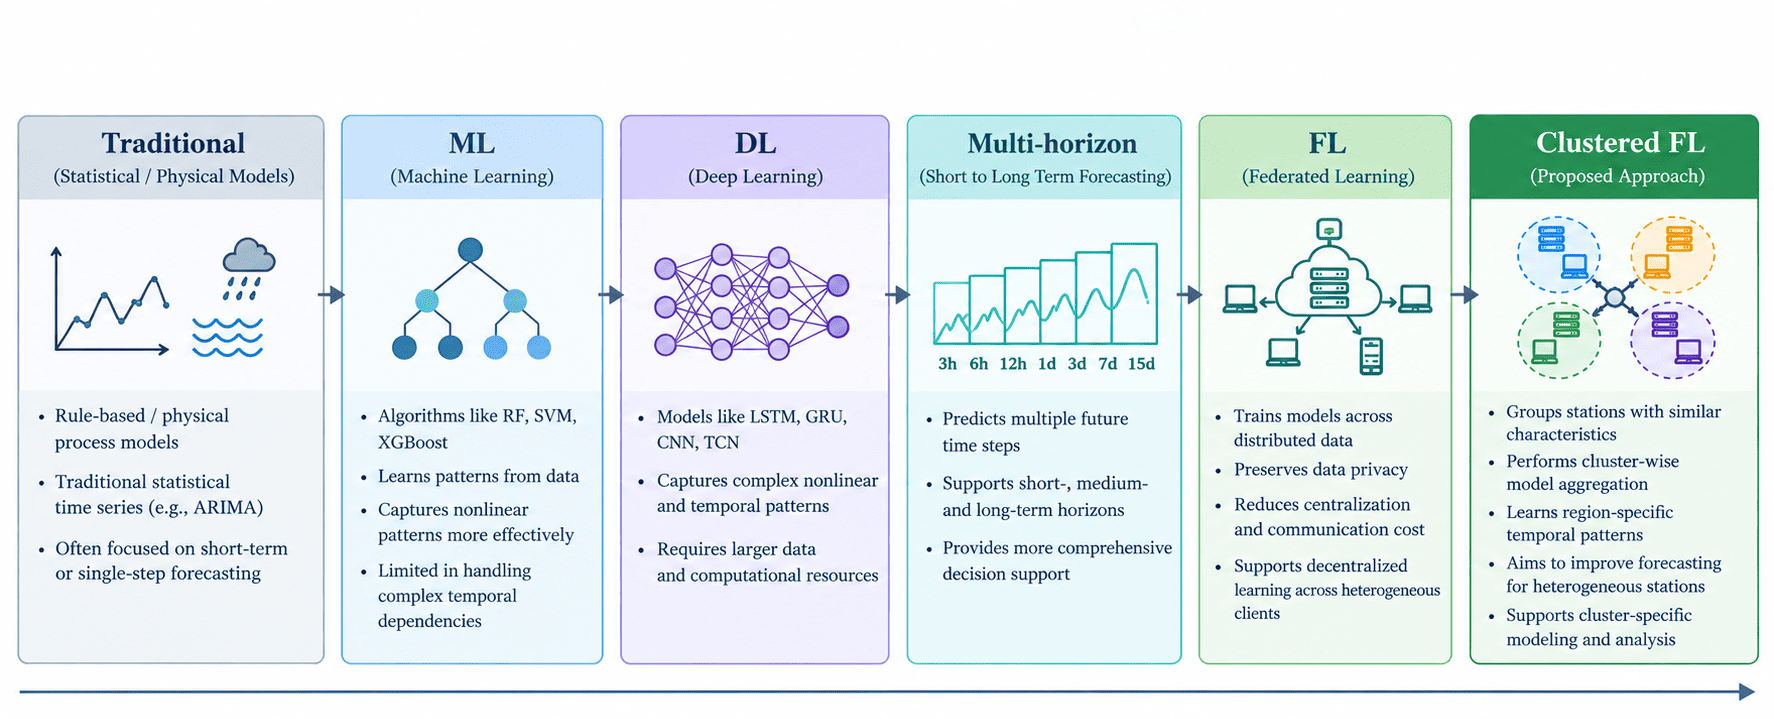
\includegraphics[width=\textwidth]{figures2/fig2_1_lit_evolution.png}
\caption{Conceptual evolution of water-level forecasting approaches, from traditional methods to the proposed CFL framework.}
\label{fig:lit-evolution}
\end{figure}

Figure~\ref{fig:lit-evolution} lays that progression out visually before the chapter walks through it section by section.

\section{Flood and Water-Level Forecasting}

Flood and water-level forecasting, in its broadest sense, means predicting future river or reservoir conditions --- water level, discharge, or the occurrence of a flood --- from historical hydrological and meteorological records, with early warning and risk management as the end goal. A systematic review covering 363 flood-prediction studies published between 2018 and 2025 found that data-driven methods, machine learning and deep learning in particular, now dominate the field across global and South Asian contexts, and, interestingly, that no single model architecture wins consistently across every study \cite{Aghenda2025}. A related review of deep-learning applications in flood forecasting reached much the same conclusion, noting that architectures ranging from feed-forward networks to convolutional and recurrent networks, along with various hybrids, have all been applied to river-flow, water-level, and flood-hazard problems, while data quality, interpretability, and computational cost remain recurring sticking points \cite{Kumar2023}.

Bangladesh has its own, fairly substantial body of work in this space, drawing mostly on records from the Bangladesh Water Development Board (BWDB) and the Bangladesh Meteorological Department (BMD), and combining hydrological and meteorological data in varying ways \cite{Islam2026a,Islam2026b,Ruma2023,Rakin2023,Rajab2023,HemelSakib2024}. Between them, these studies show that data-driven forecasting is genuinely feasible in the Bangladeshi context. What they use as input, though, differs quite a bit from one study to the next, which is where the next section picks up.

\section{Hydrological and Meteorological Data}

How much data a study actually uses, and of what kind, turns out to be one of the more telling differences across this literature --- and it is a large part of the motivation for this thesis. Some studies work from a single variable. Ruma et al. forecast water level using nothing but historical water-level records across a network of Bangladeshi river stations \cite{Ruma2023}; Islam et al., working the discharge side of things at two stations in the Old Brahmaputra basin, do much the same with discharge alone, and are upfront that leaving out meteorological variables such as precipitation is a real limitation of their study \cite{Islam2026a}.

Others combine variables. A separate study by Islam et al. brings together daily water level with rainfall and temperature at the Islampur and Sarishabari stations, using 1--5 day lag features to capture how the river responds to monsoon rainfall with a delay \cite{Islam2026b}. Cui et al. combine discharge and inflow with areal rainfall and evaporation, both computed with the Thiessen polygon method from several gauge stations \cite{Cui2022}. Rajab et al., forecasting rainfall itself as the target, use a correlation-based feature-selection step that trims an initial 18 meteorological features down to 16 \cite{Rajab2023}.

A third group skips hydrological data entirely and works only from meteorology. Rakin et al. and Hemel and Sakib both build their flood-occurrence classifiers purely from BMD weather records --- rainfall, temperature, and related variables --- with no discharge or water-level measurements involved at all \cite{Rakin2023,HemelSakib2024}. Put these three groups side by side and a fairly obvious gap appears: no Bangladeshi study reviewed here brings discharge, water level, rainfall, temperature, and evaporation together in one framework. Section 2.15 returns to this.

\section{Traditional Statistical Approaches}

Before machine learning took over, flood forecasting relied mostly on physically based hydrological models and classical statistical regression. Almost none of the literature collected for this thesis is purely statistical in that older sense --- it is nearly all machine-learning or deep-learning work --- but a couple of studies do include regression methods as part of their comparisons, and these are worth looking at for what they say about how far classical methods still get you. Rajab et al. tested Multiple Linear Regression and Polynomial Regression alongside a long list of machine-learning and deep-learning models for BMD rainfall forecasting, and found Random Forest ($R^2 = 0.768$ on the test set) and Polynomial Regression ($R^2 = 0.764$) among the stronger performers, not far off the reported LSTM results \cite{Rajab2023}. Islam et al. similarly kept Linear Regression in the mix alongside Random Forest, XGBoost, LightGBM, and LSTM when forecasting daily water level in the Old Brahmaputra basin \cite{Islam2026b}.

What this suggests, unsurprisingly, is that regression still has a place as a simple, interpretable baseline, but it tends to fall short of tree-based ensembles and deep learning once the relationships being modelled get properly nonlinear and time-dependent, which is exactly the case for hydrological data. That is the direction the rest of this chapter follows.

\section{Machine Learning-Based Forecasting}

Beyond plain regression, ensemble and kernel-based methods have been applied fairly widely to flood-related forecasting. Rakin et al. put ten machine-learning and deep-learning classifiers up against each other for Bangladesh flood occurrence, using 65 years of BMD weather data across 32 districts; LightGBM came out on top at 97.76\% accuracy, with Random Forest close behind at 97.71\% \cite{Rakin2023}. Hemel and Sakib ran a smaller comparison --- Logistic Regression, Random Forest, Gradient Boosting, XGBoost, and LSTM --- and found Gradient Boosting the strongest, at 95.38\% \cite{HemelSakib2024}.

For continuous targets, the picture is similar. Islam et al. compared Random Forest, LightGBM, and Support Vector Regression against LSTM and BiLSTM for discharge forecasting in the Old Brahmaputra basin, and while LSTM and BiLSTM ultimately came out ahead on composite performance, the tree-based and kernel-based models were not far off \cite{Islam2026a}. Hossain et al. ran a comparable comparison --- Linear Regression, Random Forest, XGBoost, MLP, LightGBM, and Polynomial Regression --- for monthly extreme water-level prediction at Islampur, using 34 years of records \cite{Hossain2025}. Perhaps the clearest single result here comes from Hameed et al., who found XGBoost beating both LSTM and Random Forest outright for monthly runoff forecasting in a glacierized catchment ($R^2 = 0.904$, NSE $= 0.797$) \cite{Hameed2025} --- a useful reminder that gradient-boosted trees are not just a fallback option when deep learning is unavailable, but a genuinely competitive method in their own right.

\section{Deep Learning for Water-Level Forecasting}

Even so, deep learning is where most of the recent activity in hydrological forecasting has gone. Aghenda et al.'s systematic review found LSTM to be the single most common architecture across the 363 studies they looked at, making up 21\% of all implementations \cite{Aghenda2025}. Kumar et al. reach a broadly similar conclusion, pointing to LSTM and GRU as particularly good at capturing temporal dependencies, with convolutional and hybrid variants such as ConvLSTM additionally able to pick up spatial patterns \cite{Kumar2023}. Waqas and Humphries explain why this works: ordinary RNNs suffer from vanishing and exploding gradients that make it hard for them to learn long-range dependencies, and LSTM's gating mechanism is specifically built to get around that \cite{Waqas2024}. The four subsections that follow look more closely at LSTM, GRU, Encoder--Decoder LSTM, and TCN in turn.

\subsection{LSTM}

Ruma et al. give a direct example of LSTM applied to Bangladesh: combined with particle swarm optimization (PSO-LSTM), their model forecasts water level across river stations on the Ganges, Brahmaputra, and Meghna, reaching an NSE of roughly 0.957 at a 15-day horizon \cite{Ruma2023}. Waqas and Humphries' review covers a much wider set of LSTM variants used in hydrology --- Bidirectional LSTM, Stacked LSTM, attention-based LSTM, and hybrids like LSTM-CNN, wavelet-LSTM, and LSTM-Transformer --- and conclude that LSTM architectures generally beat plain RNNs and GRUs on hydrological prediction, though hyperparameter sensitivity and weak generalization across different hydrological settings remain genuine problems \cite{Waqas2024}. This fits with Aghenda et al.'s finding that LSTM leads the field overall \cite{Aghenda2025}. What none of these studies do, though, is use LSTM as part of a sequence-to-sequence, multi-cluster, or federated setup --- each treats it as a single-station, single-step (or fixed-horizon) model, which is exactly the space the Encoder--Decoder and federated components of this thesis are meant to fill.

\subsection{GRU}

GRU trades some of LSTM's complexity for a simpler gating structure while still handling temporal dependencies reasonably well. Ni et al. paired GRU with TCN in a hybrid architecture that also used kernel density estimation for error bounds, and reported a 13\% RMSE reduction over standalone LSTM, GRU, and TCN \cite{Ni2024}. Li et al. included GRU as one of several baselines --- alongside RNN, LSTM, TCN, and Attention-TCN --- for streamflow forecasting in semi-arid basins, using around 20 years of daily hydrometeorological data \cite{Li2024}. Waqas and Humphries also note that GRU shows up combined with LSTM in hybrid forms elsewhere in the literature \cite{Waqas2024}. On the whole, GRU comes across as a reasonable, lighter alternative to LSTM rather than a clear improvement on it; this thesis treats it accordingly, as a baseline to compare CFL-EDLSTM against (Section 3.13) rather than as a candidate for the core architecture.

\subsection{Encoder--Decoder LSTM}

The Encoder--Decoder LSTM turns multi-step forecasting into a sequence-to-sequence problem: an encoder compresses a window of past observations into a fixed representation, and a decoder unrolls that into a sequence of future predictions. Kao et al. were among the first to apply this specifically to flood forecasting, working with hourly data from 23 typhoon events in Taiwan's Shihmen Reservoir catchment and rainfall from 10 gauge stations, forecasting reservoir inflow from one to six hours ahead. Their LSTM-ED beat a feed-forward encoder--decoder benchmark by about 3\% RMSE at the one-hour mark, and by roughly 38\% by the six-hour mark ($R^2$ around 0.98 and 0.88 respectively) --- a gap that widens with the horizon, which is itself a useful finding: the benefit of the encoder--decoder design over a simpler benchmark grows the further out you try to forecast \cite{Kao2020}.

Cui et al. took this a step further with an Encoder--Decoder that feeds an exogenous, process-model-derived forecast into the decoder (LSTM-EDE), tested across 3-, 6-, 9-, and 12-hour horizons in two Chinese basins. It came out ahead of the alternatives they compared it against, and, notably, degraded the least as the horizon lengthened, with NSE of 0.81 (Lushui) and 0.93 (Jianxi) at 12 hours \cite{Cui2022}. More recently, Lim et al. built a Seq2Seq LSTM surrogate model for real-time, multi-step flood forecasting in a coastal-urban setting and found it outperformed a standard LSTM \cite{Lim2025}, and Yuan et al. proposed a Time Residual LSTM aimed directly at fixing the degradation problem observed in Kao et al.'s original LSTM-ED baseline \cite{Kao2020,Yuan2023}. Across all four studies, the pattern holds: encoder--decoder designs consistently hold up better at longer horizons than the alternatives they are compared against. What none of them do is push past a 12-hour horizon, or train across more than one site at a time --- both of which this thesis attempts, extending the same architectural idea out to 15 days and across 26 stations grouped into four clusters.

\subsection{TCN}

The Temporal Convolutional Network takes a different route entirely, using dilated causal convolutions instead of recurrence. Lin et al. compared TCN against ANN, LSTM, and EIESM for multi-lead-time flood forecasting and found it held its own against LSTM on NSE, RMSE, and bias, though it lost ground at longer lead times \cite{Lin2021}. Li et al.'s attention-augmented version, Attention-TCN, did better still, cutting MAE by 6.9--25\% relative to a standard LSTM on heterogeneous semi-arid streamflow data \cite{Li2024}, and Ni et al.'s GRU-TCN hybrid, mentioned above, outperformed a standalone TCN as well as standalone LSTM and GRU \cite{Ni2024}. At the far end of the horizon range, Li et al. reported a hybrid combining Empirical Mode Decomposition with TCN and GRU that reached very high accuracy ($R^2 = 0.9922$, MAPE $= 3.25\%$) for 15-day streamflow forecasting, though at considerably more architectural complexity than a plain TCN \cite{Li2025}. TCN, then, is a credible non-recurrent alternative to LSTM, and it earns its place in this thesis as one of the four baseline models (Section 3.13), even though --- like the studies above --- it has not previously been tested in a multi-station or federated setting.

\section{Tree-Based Models}

Gradient-boosted decision trees sit apart from both the classical regression methods discussed in Section 2.4 and the neural architectures above, and, as already noted in Section 2.5, hold up surprisingly well in hydrological forecasting.

\subsection{XGBoost}

XGBoost in particular shows up repeatedly across this literature, both as a standalone model and as a comparison baseline. Hameed et al.'s finding that it outperforms LSTM and Random Forest for monthly runoff forecasting ($R^2 = 0.904$, NSE $= 0.797$) is probably the strongest single piece of evidence for this \cite{Hameed2025}. Within Bangladesh specifically, Hossain et al. include it among six models compared for monthly extreme water-level prediction at Islampur \cite{Hossain2025}, and Islam et al. include it in their daily water-level comparison at Islampur and Sarishabari \cite{Islam2026b}. Rakin et al. and Hemel and Sakib both use it as one of several classifiers for Bangladesh flood occurrence, with Hemel and Sakib reporting 94.47\% accuracy for it specifically \cite{Rakin2023,HemelSakib2024}. Every one of these evaluations, though, is confined to a single station or a single-site classification problem. This thesis instead runs XGBoost consistently as a baseline across all four clusters and all seven horizons (Section 3.13) --- a scale of comparison none of the studies above attempt.

\section{Multi-Horizon Forecasting}

Forecast accuracy tends to drop as the horizon lengthens, and several studies document this directly rather than just assuming it. Kao et al.'s LSTM-ED advantage over a feed-forward benchmark widened from 3\% at one hour to 38\% at six hours \cite{Kao2020}; Cui et al. found their exogenous-input design degraded the least, of the architectures they tested, up to 12 hours \cite{Cui2022}; and Yuan et al. built a Time Residual LSTM specifically to address the degradation seen in Kao et al.'s baseline at longer horizons \cite{Kao2020,Yuan2023}.

At the longer end, the evidence gets thinner but still points in a useful direction. Ruma et al. showed that 15-day water-level forecasting is achievable in Bangladesh (NSE $\approx 0.957$) \cite{Ruma2023}, and Islam et al. tested discharge forecasting across six horizons out to 30 days, finding LSTM strongest specifically at the 15- and 30-day marks \cite{Islam2026a}. Li et al.'s hybrid decomposition model reached $R^2 = 0.9922$ at a 15-day streamflow horizon \cite{Li2025}, which is a useful benchmark to keep in mind for what "good" might look like at the longest horizon considered here. None of these studies, though, evaluates one architecture across a range as wide as 3 hours to 15 days, which is precisely the design adopted in this thesis.

\section{Heterogeneity in Monitoring Stations}

There is also fairly direct evidence that station behaviour differs, sometimes considerably, even within a single river system. Islam et al. trained a discharge model at Mymensingh and tested it at the nearby Islampur station without retraining; performance held up reasonably well overall, but it varied by location and by horizon \cite{Islam2026a}. A related study by Islam et al. did much the same between Islampur and Sarishabari, again finding that how well a model transferred depended on the input scenario and the specific target station \cite{Islam2026b}. What this really shows is that even geographically close stations within the same sub-basin are different enough, statistically, for model performance to shift noticeably between them --- which is more or less the non-IID problem that federated learning research describes in general terms \cite{Zhu2021,Chen2025}, covered next.

\section{Federated Learning}

Federated learning lets distributed parties train a model together without any of them having to hand over their raw data --- a natural fit for a setting where hydrological and meteorological records are held separately by different stations or offices, as they typically are in Bangladesh.

\subsection{Conventional FL}

McMahan et al.'s Federated Averaging (FedAvg) algorithm is where this line of work begins. Clients run several rounds of local training before a central server averages their model parameters into a shared model; tested on MNIST, CIFAR-10, and language-modelling tasks, this cut the number of communication rounds needed to reach a target accuracy by roughly one to two orders of magnitude compared with plain federated SGD \cite{McMahan2017}. That basic idea --- train locally, share only the parameters, never the data --- is the mechanism this thesis borrows for training across monitoring stations. It is worth being clear, though, that FedAvg itself was built and tested on generic image and language benchmarks, under the assumption of a single shared model; it says nothing about hydrology, and nothing about what happens when the clients involved are genuinely dissimilar from one another, which is exactly the problem taken up in Section 2.10.3.

\subsection{FL for Time-Series}

Federated learning applied specifically to hydrological time series is still fairly rare, but there is at least one direct precedent. Amanzholova et al. built a federated LSTM for next-day discharge forecasting at two stations in the transboundary Chu--Talas basin, comparing it against centralized and local-only versions. At the more homogeneous of the two stations, the federated model came within about 1\% of the centralized one (NSE $0.948$ versus $0.956$); at the station with more divergent behaviour, it clearly outperformed both alternatives (NSE $0.903$, against $0.528$ centralized and $-4.230$ local-only) \cite{Amanzholova2026}. Chen et al. make a similar point more generally, using non-hydrological time-series benchmarks to show that standard federated learning struggles once client data become properly heterogeneous \cite{Chen2025}. Amanzholova et al.'s result is encouraging, but it covers only two stations, one variable, and a single one-day horizon, with no clustering involved; this thesis is, in effect, an attempt to see whether the same basic approach holds up at a rather larger scale --- 26 stations, five variables, seven horizons, and an explicit clustering step.

\subsection{Non-IID Data}

The practical difficulty with federated learning is that client data are rarely as similar to one another as the theory would like. Zhu et al.'s survey lays this out clearly: non-IID data across clients can cause slower convergence, degraded accuracy, and outright divergence under standard FedAvg, and they review a range of data-based and algorithmic fixes across both horizontal and vertical federated learning \cite{Zhu2021}. Chen et al. show much the same thing for time-series data specifically \cite{Chen2025}. This maps quite directly onto the station heterogeneity discussed in Section 2.9, where forecasting performance was shown to shift even between neighbouring stations on the same river \cite{Islam2026a,Islam2026b}. Neither Zhu et al. nor Chen et al. propose a hydrology-specific fix, though --- they describe the problem rather than solve it for this domain, which leaves the actual mitigation strategy, clustering clients before training, to the next section.

\section{Clustered and Federated Learning}

Clustered Federated Learning takes a fairly intuitive approach to the non-IID problem: instead of forcing every client into one shared model, group clients that look similar and train a model per group. Ghosh et al.'s Iterative Federated Clustering Algorithm (IFCA) does this by repeatedly estimating which cluster each client belongs to and updating that cluster's model accordingly, and it clearly beats both a single global model and fully local training on heterogeneous benchmarks --- 95.25\% accuracy versus 89.73\% and 80.05\% on a four-cluster Rotated MNIST setup, and 81.51\% versus 77.87\% and 33.97\% on a two-cluster Rotated CIFAR setup \cite{Ghosh2021}.

Harshvardhan et al.'s Successive Refine Federated Clustering Algorithm (SR-FCA) improves on this in one important way: it does not need to know the number of clusters in advance, unlike IFCA. It also comes out ahead of Local, Global, and IFCA baselines across several benchmarks --- 92.84\% on inverted MNIST, 91.83\% on rotated MNIST, 88.70\% on rotated CIFAR-10, and 84.93\% on FEMNIST \cite{Harshvardhan2022}. Ben Ali et al. step back from individual algorithms and organize the field into a taxonomy --- server-side clustering (based on model weights or gradients), client-side clustering (based on training loss or model selection), and metadata-based clustering (based on shared statistical descriptors) --- while pointing out that cluster-quality metrics such as the Adjusted Rand Index, Cluster Purity, and Silhouette Score exist but that choosing the right number of clusters in the first place remains an open problem \cite{BenAli2026}.

None of these three studies has anything to do with hydrology; all of them rely on image or text benchmarks with artificially constructed heterogeneity. That leaves an obvious question unanswered: what does a "cluster" even mean when the clients are river-monitoring stations rather than benchmark partitions? The CFL literature clusters clients by model similarity or by statistical metadata; this thesis instead defines its four clusters --- Upstream, Middle, Downstream, Urban --- using hydrological domain knowledge, an approach none of the algorithms above were tested against.

\section{Explainable AI}

The more accurate hydrological forecasting models have become, the more it has mattered that someone can actually explain their predictions, particularly where those predictions feed into early-warning decisions. Khorrami et al. reviewed 83 studies applying explainable AI to runoff and water-level forecasting, spanning both ante-hoc and post-hoc methods across several model types including LSTM, and their headline finding is that SHAP is, by a clear margin, the dominant post-hoc method in this space \cite{Khorrami2025}.

\subsection{SHAP}

SHAP itself, introduced by Lundberg and Lee, gives a theoretically grounded way of attributing a model's output to its individual input features. It unifies a number of earlier feature-attribution methods and proves that the resulting Shapley-value attribution is the only one satisfying three desirable properties --- local accuracy, missingness, and consistency; the original paper also shows SHAP to be more sample-efficient than LIME and Shapley sampling across several model types, including a CNN \cite{Lundberg2017}. It was never built with hydrology in mind, but being model-agnostic, it applies just as well there as anywhere else.

Huang et al. put this into practice, integrating SHAP (via a Gradient Explainer) into a coupled CNN-LSTM flood model for the Beijiang River Basin, built from rainfall and runoff data at 17 stations. Their model reached NSE $= 0.838$ at a 25-hour horizon, ahead of standalone CNN (0.737) and LSTM (0.745), and the SHAP analysis found that recent downstream runoff dominated the predictions, with rainfall contributing comparatively little \cite{Huang2024}. Hemel and Sakib applied SHAP and LIME together to a Gradient Boosting flood classifier for Bangladesh and identified rainfall as a particularly strong predictor \cite{HemelSakib2024}. Parasar et al. used SHAP on a hydroclimatic discharge model in a monsoon-dominated river system, and were able to show how the relative influence of rainfall versus antecedent discharge shifted under monsoon conditions not unlike those found in Bangladesh \cite{Parasar2025}. None of these three applications, though, sits inside a clustered or federated model, and none asks whether feature importance actually looks different from one part of a river network to another. That is exactly the question this thesis puts to SHAP in Section 3.16 --- computing it separately for each of the four clusters, rather than once for the whole network, to see whether the patterns Huang et al. and Parasar et al. found at single sites hold consistently, or not, across Upstream, Middle, Downstream, and Urban stations.

\section{Visualization and Decision-Support Systems}

This is, honestly, the thinnest part of the literature collected for this thesis. Lim et al.'s Seq2Seq LSTM surrogate model was explicitly built with real-time, operational use in mind for a coastal-urban flood context \cite{Lim2025}, which at least signals that practical, decision-relevant delivery is a recognized concern, even if it is rarely the main focus of a study. A number of the Bangladesh-focused papers gesture in this direction without quite getting there: Ruma et al. and Islam et al. both flag real-time, operationally grounded forecasting as a natural next step for their work \cite{Islam2026a,Ruma2023}, and Hemel and Sakib note that their classification-based approach does not incorporate real-time hydrological data \cite{HemelSakib2024}. This thesis addresses that gap fairly directly, by building an interactive web-based visualization interface (Chapter 3) that presents station-level forecasts and sets them alongside water-level information published by the FFWC, used here as an external point of comparison rather than as a validated ground truth.

\section{Critical Comparison of Existing Studies}

Stepping back, the literature reviewed in this chapter falls into four groups that, so far, have not had much to do with one another. Bangladesh-specific forecasting studies work with a single data modality at a time, ranging from a handful of specific hydrological stations to much larger pooled networks of stations or districts, but always in a centralized setting \cite{Islam2026a,Islam2026b,Ruma2023,Rakin2023,Rajab2023,HemelSakib2024,Hossain2025}. Deep-learning architecture research --- Encoder--Decoder LSTM, TCN, gradient-boosted trees --- establishes strong methods for multi-step forecasting, but almost entirely outside Bangladesh and always in a centralized setup \cite{Kao2020,Cui2022,Lim2025,Yuan2023,Ni2024,Kumar2023,Hameed2025,Waqas2024,Aghenda2025,Li2024,Lin2021,Li2025}. Federated and clustered federated learning research shows that FedAvg and cluster-specific training deal with client heterogeneity reasonably well, but only on generic benchmarks or, at most, a two-station hydrological case \cite{McMahan2017,Zhu2021,Chen2025,Ghosh2021,Harshvardhan2022,BenAli2026,Amanzholova2026}. And explainable-AI research has established SHAP as the go-to interpretability method for hydrological deep learning, without yet putting it inside a clustered or federated model \cite{Lundberg2017,Huang2024,Khorrami2025,Parasar2025}.

Table~\ref{tab:lit-comparison} lays this out more concretely, showing where each strand sits on data modality, scale and architecture, and its main limitation as far as this thesis is concerned.

\vspace{-0.3cm}
\begin{table}[htbp]
\centering
\caption{Critical comparison of the four reviewed research strands}
\label{tab:lit-comparison}
\small
\setlength{\tabcolsep}{4pt}
\renewcommand{\arraystretch}{1.25}

\begin{tabularx}{\textwidth}{
    >{\raggedright\arraybackslash}p{3.0cm}
    >{\raggedright\arraybackslash}X
    >{\raggedright\arraybackslash}X
    >{\raggedright\arraybackslash}X
}
\toprule
\textbf{Research Strand} &
\textbf{Data Modality} &
\textbf{Scale / Architecture} &
\textbf{Key Limitation} \\
\midrule

\textbf{Bangladesh-specific forecasting}
\cite{Islam2026a,Islam2026b,Ruma2023,Rakin2023,Rajab2023,HemelSakib2024,Hossain2025}
&
Single or limited data modality, including water level, discharge, rainfall, and meteorological variables
&
Ranges from 1--3 specific stations to large pooled networks (20+ stations or districts), but always trained as a single centralized model
&
No multivariate (hydrological + meteorological) integration and no cluster-specific or federated modeling, regardless of network size
\\[0.8em]

\textbf{Deep-learning architectures}
\cite{Kao2020,Cui2022,Lim2025,Yuan2023,Ni2024,Li2024,Lin2021,Li2025}
&
Hydrological and hydro-meteorological time-series data, mainly from non-Bangladesh studies
&
Mostly centralized forecasting at individual sites or datasets using LSTM, GRU, Encoder--Decoder LSTM, TCN, and related architectures
&
Limited evaluation in distributed or federated multi-station hydrological forecasting
\\[0.8em]

\textbf{Federated / Clustered Federated Learning}
\cite{McMahan2017,Zhu2021,Chen2025,Ghosh2021,Harshvardhan2022,BenAli2026,Amanzholova2026}
&
Benchmark datasets and limited hydrological applications
&
Distributed clients using federated, clustered, or personalized aggregation approaches
&
Limited application to multi-station, multi-horizon hydrological forecasting with heterogeneous stations
\\[0.8em]

\textbf{Explainable AI}
\cite{Lundberg2017,Huang2024,Khorrami2025,Parasar2025}
&
Hydrological and hydro-climatic forecasting or classification data
&
Mainly centralized models using SHAP, LIME, and related feature-attribution methods
&
Generally not integrated with federated or clustered federated learning across heterogeneous stations
\\

\bottomrule
\end{tabularx}
\end{table}
\vspace{-0.3cm}

\section{Research Gap}

No study identified in this review brings all four of these strands together: multivariate inputs (discharge, water level, rainfall, temperature, evaporation), a multi-station, multi-cluster network (26 stations across four hydrologically defined groups), a wide range of horizons (3 hours to 15 days), federated and cluster-aware training, and SHAP-based interpretation, compared against an external reference (FFWC) through an accessible visualization platform. More specifically:

\begin{itemize}
    \item No Bangladesh-focused study combines all five hydrometeorological variables used in this thesis within a single forecasting framework (Section 2.3).
    \item No reviewed study tests one architecture across a horizon range as wide as 3 hours to 15 days (Section 2.8).
    \item No reviewed study applies clustered federated learning --- as distinct from a single global federated model, or a purely centralized cross-station transfer-learning setup --- to a hydrological forecasting network (Sections 2.9--2.11).
    \item No reviewed study applies SHAP within a clustered or federated hydrological model, or compares feature importance across hydrologically distinct station clusters (Section 2.12).
    \item Dedicated visualization or decision-support tooling for Bangladesh water-level forecasting, compared against an external reference such as the FFWC, is largely absent from the literature identified in this review (Section 2.13).
\end{itemize}

Chapter 3 sets out the CFL-EDLSTM framework built to address this gap.

\section{Summary}

This chapter moved from the general problem of flood and water-level forecasting, and the hydrological and meteorological data used to tackle it, through traditional statistical and machine-learning methods, into the deep-learning architectures --- Vanilla LSTM, GRU, Encoder--Decoder LSTM, and TCN --- and tree-based models that are most relevant to this thesis. It then turned to multi-horizon forecasting and station heterogeneity, which together motivate the case for federated and, more specifically, clustered federated learning, before covering explainable AI, and SHAP in particular, as a way of making the resulting models interpretable. A critical comparison of these four strands --- Bangladesh-specific forecasting, deep-learning architectures, federated/clustered learning, and explainable AI --- showed that they have, so far, developed largely in isolation from one another. The chapter closed by setting out, precisely, where that leaves an opening: a multivariate, multi-cluster, multi-horizon, federated, and interpretable forecasting framework for Bangladesh, which is what Chapter 3 now sets out to build.